\begin{center}\emph{Introduction}\end{center}

Decentralised finance (DeFi) is the longstanding vision of a truly global and borderless financial system, the promise of universal, low-cost access to banking services and international financial markets, eliminating geographic and socio-political barriers of entry and reliance upon centralised financial institutions, subverting the power-base of monopolistic and hegemonic access to capital, facilitating a highly competitive global economic landscape.

Smart-contracts enabling arbitrary, self-executing algorithmic exchange facilitate the synthesis of sophisticated financial instruments in the absence of conventional centralised exchanges. The algorithmic versatility of smart-contracts affords their use as a primitive in the construction of sophisticated distributed protocols such as Decentralised Autonomous Organisations (DAOs).

%The key characteristics of DeFi are \cite{???,EthereumDevs}:
%\begin{itemize}
%	\item Non-custodial: users assert full control over their own assets.
%	\item Open: protocols are borderless and globally accessible.
%	\item Transparency: protocols and algorithms are open-source.
%	\item Composable: code may be modularised and layered, enabling thriving development and innovation of the ecosystem.
%	\item Decentralised: the absence of top-down control and centralisation of power.
%\end{itemize}

\begin{center}\emph{Consensus}\end{center}

In a decentralised environment transactions are approved via \emph{consensus} (Sec.~\ref{sec:consensus}), whereby a small number of randomly chosen network nodes form \emph{consensus sets}, collectively acting as delegates for the network to authorise transactions by majority vote. Consensus outcomes should with high probability reflect the network majority, a function of consensus set size and the ratio of dishonest nodes.

\begin{center}
	\vspace{2pt}
	\resizebox{0.6\columnwidth}{!}{\tdplotsetmaincoords{70}{110}
\begin{tikzpicture}[genericStyle, tdplot_main_coords]
	\def\radiusN{0.3}
	\def\radiusC{0.4}
    \draw[nodeConsensusLightStyle] (1, 1, 0) circle (\radiusN);
    \draw[draw=nodeConsensusLineColor] (1,1,0) -- (3,3,2.5);
    \draw[nodeNetworkLightStyle] (1, 2, 0) circle (\radiusN);
    \draw[nodeNetworkLightStyle] (1, 3, 0) circle (\radiusN);
    \draw[nodeConsensusLightStyle] (1, 4, 0) circle (\radiusN);
    \draw[draw=nodeConsensusLineColor] (1,4,0) -- (3,3,2.5);
    \draw[nodeNetworkLightStyle] (1, 5, 0) circle (\radiusN);
    \draw[nodeNetworkLightStyle] (2, 1, 0) circle (\radiusN);
    \draw[nodeNetworkLightStyle] (2, 2, 0) circle (\radiusN);
    \draw[nodeNetworkLightStyle] (2, 3, 0) circle (\radiusN);
    \draw[nodeNetworkLightStyle] (2, 4, 0) circle (\radiusN);
    \draw[nodeNetworkLightStyle] (2, 5, 0) circle (\radiusN);
    \draw[nodeNetworkLightStyle] (3, 1, 0) circle (\radiusN);
    \draw[nodeNetworkLightStyle] (3, 2, 0) circle (\radiusN);
    \draw[nodeNetworkLightStyle] (3, 3, 0) circle (\radiusN);
    \draw[nodeNetworkLightStyle] (3, 4, 0) circle (\radiusN);
    \draw[nodeNetworkLightStyle] (3, 5, 0) circle (\radiusN);
    \draw[nodeNetworkLightStyle] (4, 1, 0) circle (\radiusN);
    \draw[nodeConsensusLightStyle] (4, 2, 0) circle (\radiusN);
    \draw[draw=nodeConsensusLineColor] (4,2,0) -- (3,3,2.5);
    \draw[nodeNetworkLightStyle] (4, 3, 0) circle (\radiusN);
    \draw[nodeNetworkLightStyle] (4, 4, 0) circle (\radiusN);
    \draw[nodeConsensusLightStyle] (4, 5, 0) circle (\radiusN);
    \draw[draw=nodeConsensusLineColor] (4,5,0) -- (3,3,2.5);
    \draw[nodeNetworkLightStyle] (5, 1, 0) circle (\radiusN);
    \draw[nodeNetworkLightStyle] (5, 2, 0) circle (\radiusN);
    \draw[nodeNetworkLightStyle] (5, 3, 0) circle (\radiusN);
    \draw[nodeConsensusLightStyle] (5, 4, 0) circle (\radiusN);
    \draw[draw=nodeConsensusLineColor] (5,4,0) -- (3,3,2.5);
    \draw[nodeNetworkLightStyle] (5, 5, 0) circle (\radiusN);
    \draw[nodeConsensusLightStyle] (3, 3, 2.5) circle (\radiusC);
    
    \coordinate (originN) at (3,3,0);
    \coordinate (originC) at (3,3,2.5);
    
    \node[draw=none, text=black] at ([shift={(2.25em,0)}]originC) {\large $\mathcal{C}$};
    \node[draw=none, text=black] at ([shift={(7.5em,-1.5em)}]originN) {\large $\mathcal{N}$};
\end{tikzpicture}
}
\end{center}

The randomisation of nodes forming consensus is vital to ensure the integrity of consensus outcomes (Sec.~\ref{sec:random_subset_problem}). If the choice of consensus nodes were known in advance this would provide avenues for malicious parties to compromise security by targeting the known allocation. Randomisation effectively erases assignment information, eliminating all avenues for strategic alignment.

\begin{center}
	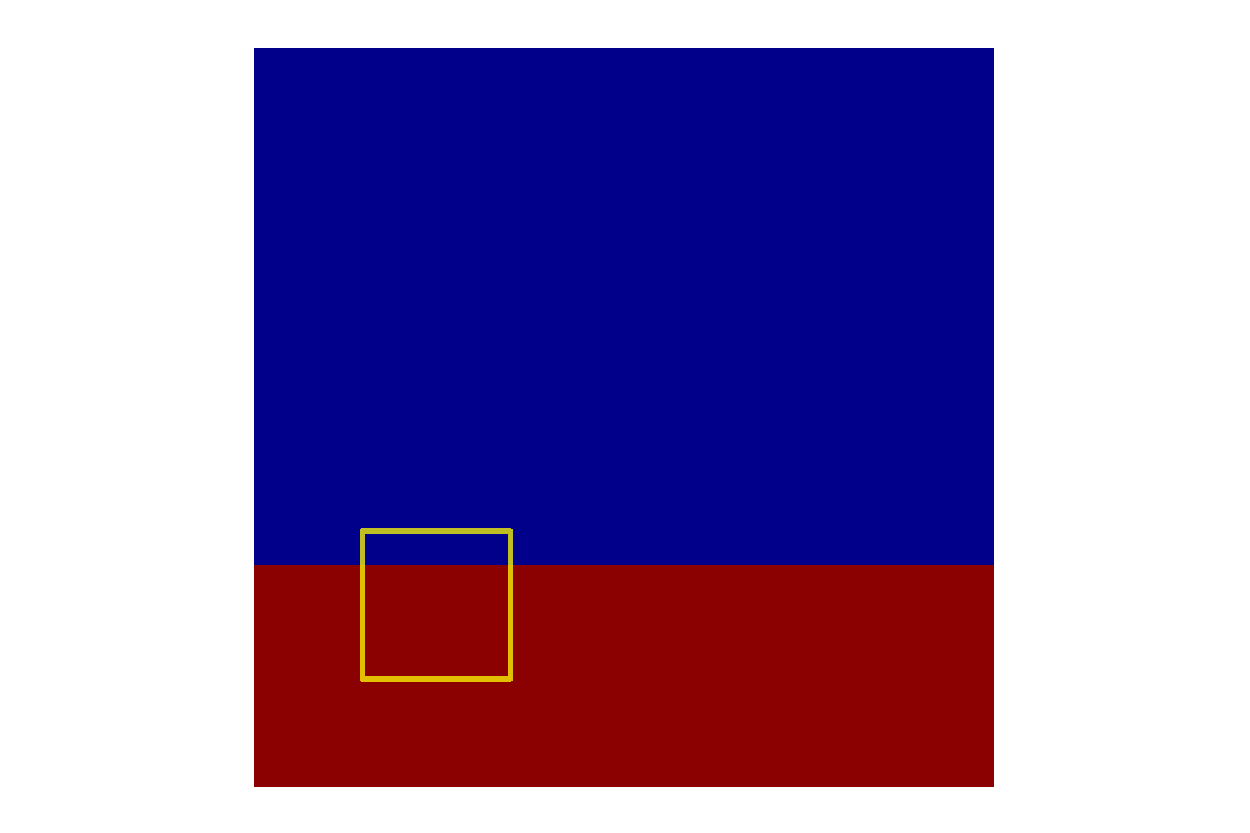
\includegraphics[width=0.4\columnwidth]{figs/strategy_entropy_S_p03.pdf}
	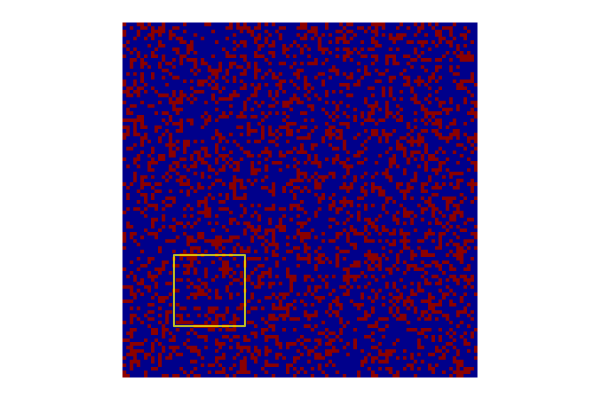
\includegraphics[width=0.4\columnwidth]{figs/strategy_entropy_R_p03.pdf}
\end{center}

Distributed algorithms for assigning consensus sets must be secure in the sense that their randomisation cannot be compromised by malicious parties.

\begin{center}\emph{Proof-of-work}\end{center}

The Bitcoin protocol \cite{Nakamoto08} first introduced proof-of-work (PoW) as mechanism for securely randomly selecting a small number of network nodes at random to form consensus (Sec.~\ref{sec:PoW}). This protocol operates in the context of a network of unknown and unidentifiable nodes in which anyone may freely participate. The algorithm requires nodes to compete to solve inverse-hashing problems, a randomised algorithm that effectively chooses winners by lottery.

While the proof-of-work mining algorithm provides an ingenious solution to the random subset problem it is highly inefficient, resulting in enormous net energy consumption to maintain the network. Currently, annualised energy consumption of the Bitcoin network is $\sim$155TWh \cite{CBECI}\footnote{Estimate as of January 19, 2024.}, comparable to the total electricity consumption of medium sized countries\footnote{Estimated annual electricity consumption of Sweden (2022): $\sim$164TWh.}.

The inefficiency of proof-of-work presents a significant obstacle for scalability, motivating the development of more efficient alternate consensus algorithms. Proof-of-stake (PoS) \cite{KingNadal, Bentov} is a leading alternative, recently adopted by the Ethereum network to improve scalability and reduce transaction costs. Ethereum's \cite{Buterin} transition to proof-of-stake, famously known as \emph{The Merge}, reduced its annualised energy consumption from $\sim$21TWh (PoW) to $\sim$2GWh (PoS) \cite{CBECI}\footnote{Estimates immediately prior and subsequent to \emph{The Merge} on September 15, 2022.}, a spontaneous reduction in energy consumption of 99.99\%. However, despite its radically improved energy efficiency, proof-of-stake has been criticised for affording reduced security owing to its increased vulnerability to manipulation and reduced level of randomisation. Proof-of-work based on quantum sampling problems has also been investigated as a means for enhanced energy efficiency \cite{QPoW}.

%\begin{center}
%	\includegraphics[width=0.9\columnwidth]{figs/bitcoin_energy_consumption.pdf}
%\end{center}

\begin{center}\emph{Network structure}\end{center}

* Anonymous vs identifiable nodes

* Open vs closed

* Random subset problem

* Key establishment

\begin{center}\emph{Consensus assignment problem}\end{center}

Networks comprising known nodes afford more efficient distributed algorithms for solving the random subset problem. By utilising secure shared randomness (Sec.~\ref{sec:secure_shared_randomness}) all network nodes may be simultaneously allocated to random subsets (Sec.~\ref{sec:hash_based_random_subsets}), ensuring full resource utilisation.

The generalisation of the random subset problem is the \emph{consensus assignment problem} (Sec.~\ref{sec:consensus_assignment_problem}), enabling the simultaneous allocation of network nodes to consensus sets.

\begin{center}
	\resizebox{!}{0.5\columnwidth}{\input{figs/intro_bipartite.tex}}
	\hspace{1.5em}
	\resizebox{!}{0.5\columnwidth}{%\resizebox{0.31\columnwidth}{!}{
    \begin{tikzpicture}[genericStyle]
        \def\N{6}
        \def\nskip{8}
        \def\conn{3}
        \def\UVsep{2.8}

        \foreach \i in {1,...,\N} {
                \ifnum\i=\nskip
                    \node[draw=none] (a\i) at (0,-\i) {\LARGE $\vdots$};
                \else
                    \ifnum\i=\N
                        \node[nodeNetworkStyle] (a\i) at (0,-\i) {}; % $u_m$
                    \else
                        \node[nodeNetworkStyle] (a\i) at (0,-\i) {}; % $u_{\i}$
                    \fi
                \fi
            }
        \foreach \i in {1,...,\N} {
                \ifnum\i=\nskip
                    \node[draw=none] (b\i) at (\UVsep,-\i) {\LARGE $\vdots$};
                \else
                    \ifnum\i=\N
                        \node[nodeConsensusStyle] (b\i) at (\UVsep,-\i) {}; % $v_n$
                    \else
                        \node[nodeConsensusStyle] (b\i) at (\UVsep,-\i) {}; % $v_{\i}$
                    \fi
                \fi
            }

        \foreach \i in {1,...,\N} {
                \foreach \j in {1,...,\N} {
                        \ifnum\i=\nskip
                        \else
                            \ifnum\j=\nskip
                            \else
                                \draw[graphNonEdgeStyle] ($(a\i.east)$) -- ($(b\j.west)$);
                            \fi
                        \fi
                    }
            }

        \draw[graphEdgeStyle] ($(a1.east)$) -- ($(b2.west)$);
        \draw[graphEdgeStyle] ($(a1.east)$) -- ($(b4.west)$);
        \draw[graphEdgeStyle] ($(a1.east)$) -- ($(b6.west)$);

        \draw[graphEdgeStyle] ($(a2.east)$) -- ($(b1.west)$);
        \draw[graphEdgeStyle] ($(a2.east)$) -- ($(b3.west)$);
        \draw[graphEdgeStyle] ($(a2.east)$) -- ($(b5.west)$);

        \draw[graphEdgeStyle] ($(a3.east)$) -- ($(b4.west)$);
        \draw[graphEdgeStyle] ($(a3.east)$) -- ($(b5.west)$);
        \draw[graphEdgeStyle] ($(a3.east)$) -- ($(b6.west)$);

        \draw[graphEdgeStyle] ($(a4.east)$) -- ($(b1.west)$);
        \draw[graphEdgeStyle] ($(a4.east)$) -- ($(b2.west)$);
        \draw[graphEdgeStyle] ($(a4.east)$) -- ($(b3.west)$);

        \draw[graphEdgeStyle] ($(a5.east)$) -- ($(b2.west)$);
        \draw[graphEdgeStyle] ($(a5.east)$) -- ($(b3.west)$);
        \draw[graphEdgeStyle] ($(a5.east)$) -- ($(b4.west)$);

        \draw[graphEdgeStyle] ($(a6.east)$) -- ($(b1.west)$);
        \draw[graphEdgeStyle] ($(a6.east)$) -- ($(b5.west)$);
        \draw[graphEdgeStyle] ($(a6.east)$) -- ($(b6.west)$);

     \node[draw=none, text=black] (labelX) at ($(a1)!0.5!(b1) + (0,0.65)$) {\Large $\mathcal{X}_\mathcal{N}$};

    \end{tikzpicture}
%}}
\end{center}

\begin{center}\emph{Distributed consensus networks}\end{center}

Distributed consensus networks (DCNs) combine the consensus assignment problem with an economic model that self-incentivises the honest participation of nodes (Sec.~\ref{sec:DCN}). The product of DCNs is proofs-of-consensus (PoC) --- timestamped, cryptographic proofs that a sets of nodes form secure random subsets of a network established via distributed execution of the consensus assignment problem (Sec.~\ref{sec:PoC}).

DCNs treat consensus as an abstract market commodity, an enabler of generic digital trade. The internal operation of DCNs is inherently non-monetary, a barter economy in which nodes contribute to consensus load in equal exchange for the consensus load they request. Nodes act as gateways to the DCNs to which they belong, and may independently utilise and monetise consensus load, collectively facilitating an externally-facing competitive bidding market for consensus (Sec.~\ref{sec:economics}).

\begin{center}
	\resizebox{0.8\columnwidth}{!}{\tdplotsetmaincoords{70}{110}

\begin{tikzpicture}[scale=2.5, tdplot_main_coords]
\def\vOff{4}
\def\myRad{0.02}
\def\myLW{0.25}
\def\myHeight{0.75}
\def\lineOp{0.075}
% Nodes
\draw[draw=blue, line width=\myLW, fill=cyan!20] (-0.5, -0.5, 0) circle (\myRad) coordinate(n1);
\draw[draw=blue, line width=\myLW, fill=cyan!20] (-0.5, -0.42857142857142855, 0) circle (\myRad) coordinate(n16);
\draw[draw=blue, line width=\myLW, fill=cyan!20] (-0.5, -0.35714285714285715, 0) circle (\myRad) coordinate(n31);
\draw[draw=blue, line width=\myLW, fill=cyan!20] (-0.5, -0.2857142857142857, 0) circle (\myRad) coordinate(n46);
\draw[draw=blue, line width=\myLW, fill=cyan!20] (-0.5, -0.21428571428571427, 0) circle (\myRad) coordinate(n61);
\draw[draw=blue, line width=\myLW, fill=cyan!20] (-0.5, -0.14285714285714285, 0) circle (\myRad) coordinate(n76);
\draw[draw=red, line width=\myLW, fill=red!20] (-0.5, -0.07142857142857142, 0) circle (\myRad) coordinate(n91);
\draw[draw=blue, line width=\myLW, fill=cyan!20] (-0.5, 0.0, 0) circle (\myRad) coordinate(n106);
\draw[draw=red, line width=\myLW, fill=red!20] (-0.5, 0.07142857142857142, 0) circle (\myRad) coordinate(n121);
\draw[draw=blue, line width=\myLW, fill=cyan!20] (-0.5, 0.14285714285714285, 0) circle (\myRad) coordinate(n136);
\draw[draw=blue, line width=\myLW, fill=cyan!20] (-0.5, 0.21428571428571427, 0) circle (\myRad) coordinate(n151);
\draw[draw=red, line width=\myLW, fill=red!20] (-0.5, 0.2857142857142857, 0) circle (\myRad) coordinate(n166);
\draw[draw=blue, line width=\myLW, fill=cyan!20] (-0.5, 0.35714285714285715, 0) circle (\myRad) coordinate(n181);
\draw[draw=blue, line width=\myLW, fill=cyan!20] (-0.5, 0.42857142857142855, 0) circle (\myRad) coordinate(n196);
\draw[draw=blue, line width=\myLW, fill=cyan!20] (-0.5, 0.5, 0) circle (\myRad) coordinate(n211);
\draw[draw=red, line width=\myLW, fill=red!20] (-0.42857142857142855, -0.5, 0) circle (\myRad) coordinate(n2);
\draw[draw=blue, line width=\myLW, fill=cyan!20] (-0.42857142857142855, -0.42857142857142855, 0) circle (\myRad) coordinate(n17);
\draw[draw=blue, line width=\myLW, fill=cyan!20] (-0.42857142857142855, -0.35714285714285715, 0) circle (\myRad) coordinate(n32);
\draw[draw=blue, line width=\myLW, fill=cyan!20] (-0.42857142857142855, -0.2857142857142857, 0) circle (\myRad) coordinate(n47);
\draw[draw=blue, line width=\myLW, fill=cyan!20] (-0.42857142857142855, -0.21428571428571427, 0) circle (\myRad) coordinate(n62);
\draw[draw=blue, line width=\myLW, fill=cyan!20] (-0.42857142857142855, -0.14285714285714285, 0) circle (\myRad) coordinate(n77);
\draw[draw=blue, line width=\myLW, fill=cyan!20] (-0.42857142857142855, -0.07142857142857142, 0) circle (\myRad) coordinate(n92);
\draw[draw=red, line width=\myLW, fill=red!20] (-0.42857142857142855, 0.0, 0) circle (\myRad) coordinate(n107);
\draw[draw=blue, line width=\myLW, fill=cyan!20] (-0.42857142857142855, 0.07142857142857142, 0) circle (\myRad) coordinate(n122);
\draw[draw=blue, line width=\myLW, fill=cyan!20] (-0.42857142857142855, 0.14285714285714285, 0) circle (\myRad) coordinate(n137);
\draw[draw=blue, line width=\myLW, fill=cyan!20] (-0.42857142857142855, 0.21428571428571427, 0) circle (\myRad) coordinate(n152);
\draw[draw=blue, line width=\myLW, fill=cyan!20] (-0.42857142857142855, 0.2857142857142857, 0) circle (\myRad) coordinate(n167);
\draw[draw=blue, line width=\myLW, fill=cyan!20] (-0.42857142857142855, 0.35714285714285715, 0) circle (\myRad) coordinate(n182);
\draw[draw=blue, line width=\myLW, fill=cyan!20] (-0.42857142857142855, 0.42857142857142855, 0) circle (\myRad) coordinate(n197);
\draw[draw=blue, line width=\myLW, fill=cyan!20] (-0.42857142857142855, 0.5, 0) circle (\myRad) coordinate(n212);
\draw[draw=red, line width=\myLW, fill=red!20] (-0.35714285714285715, -0.5, 0) circle (\myRad) coordinate(n3);
\draw[draw=blue, line width=\myLW, fill=cyan!20] (-0.35714285714285715, -0.42857142857142855, 0) circle (\myRad) coordinate(n18);
\draw[draw=red, line width=\myLW, fill=red!20] (-0.35714285714285715, -0.35714285714285715, 0) circle (\myRad) coordinate(n33);
\draw[draw=blue, line width=\myLW, fill=cyan!20] (-0.35714285714285715, -0.2857142857142857, 0) circle (\myRad) coordinate(n48);
\draw[draw=blue, line width=\myLW, fill=cyan!20] (-0.35714285714285715, -0.21428571428571427, 0) circle (\myRad) coordinate(n63);
\draw[draw=blue, line width=\myLW, fill=cyan!20] (-0.35714285714285715, -0.14285714285714285, 0) circle (\myRad) coordinate(n78);
\draw[draw=blue, line width=\myLW, fill=cyan!20] (-0.35714285714285715, -0.07142857142857142, 0) circle (\myRad) coordinate(n93);
\draw[draw=blue, line width=\myLW, fill=cyan!20] (-0.35714285714285715, 0.0, 0) circle (\myRad) coordinate(n108);
\draw[draw=blue, line width=\myLW, fill=cyan!20] (-0.35714285714285715, 0.07142857142857142, 0) circle (\myRad) coordinate(n123);
\draw[draw=blue, line width=\myLW, fill=cyan!20] (-0.35714285714285715, 0.14285714285714285, 0) circle (\myRad) coordinate(n138);
\draw[draw=blue, line width=\myLW, fill=cyan!20] (-0.35714285714285715, 0.21428571428571427, 0) circle (\myRad) coordinate(n153);
\draw[draw=blue, line width=\myLW, fill=cyan!20] (-0.35714285714285715, 0.2857142857142857, 0) circle (\myRad) coordinate(n168);
\draw[draw=red, line width=\myLW, fill=red!20] (-0.35714285714285715, 0.35714285714285715, 0) circle (\myRad) coordinate(n183);
\draw[draw=blue, line width=\myLW, fill=cyan!20] (-0.35714285714285715, 0.42857142857142855, 0) circle (\myRad) coordinate(n198);
\draw[draw=blue, line width=\myLW, fill=cyan!20] (-0.35714285714285715, 0.5, 0) circle (\myRad) coordinate(n213);
\draw[draw=blue, line width=\myLW, fill=cyan!20] (-0.2857142857142857, -0.5, 0) circle (\myRad) coordinate(n4);
\draw[draw=blue, line width=\myLW, fill=cyan!20] (-0.2857142857142857, -0.42857142857142855, 0) circle (\myRad) coordinate(n19);
\draw[draw=red, line width=\myLW, fill=red!20] (-0.2857142857142857, -0.35714285714285715, 0) circle (\myRad) coordinate(n34);
\draw[draw=red, line width=\myLW, fill=red!20] (-0.2857142857142857, -0.2857142857142857, 0) circle (\myRad) coordinate(n49);
\draw[draw=blue, line width=\myLW, fill=cyan!20] (-0.2857142857142857, -0.21428571428571427, 0) circle (\myRad) coordinate(n64);
\draw[draw=blue, line width=\myLW, fill=cyan!20] (-0.2857142857142857, -0.14285714285714285, 0) circle (\myRad) coordinate(n79);
\draw[draw=blue, line width=\myLW, fill=cyan!20] (-0.2857142857142857, -0.07142857142857142, 0) circle (\myRad) coordinate(n94);
\draw[draw=red, line width=\myLW, fill=red!20] (-0.2857142857142857, 0.0, 0) circle (\myRad) coordinate(n109);
\draw[draw=blue, line width=\myLW, fill=cyan!20] (-0.2857142857142857, 0.07142857142857142, 0) circle (\myRad) coordinate(n124);
\draw[draw=blue, line width=\myLW, fill=cyan!20] (-0.2857142857142857, 0.14285714285714285, 0) circle (\myRad) coordinate(n139);
\draw[draw=red, line width=\myLW, fill=red!20] (-0.2857142857142857, 0.21428571428571427, 0) circle (\myRad) coordinate(n154);
\draw[draw=red, line width=\myLW, fill=red!20] (-0.2857142857142857, 0.2857142857142857, 0) circle (\myRad) coordinate(n169);
\draw[draw=red, line width=\myLW, fill=red!20] (-0.2857142857142857, 0.35714285714285715, 0) circle (\myRad) coordinate(n184);
\draw[draw=red, line width=\myLW, fill=red!20] (-0.2857142857142857, 0.42857142857142855, 0) circle (\myRad) coordinate(n199);
\draw[draw=blue, line width=\myLW, fill=cyan!20] (-0.2857142857142857, 0.5, 0) circle (\myRad) coordinate(n214);
\draw[draw=red, line width=\myLW, fill=red!20] (-0.21428571428571427, -0.5, 0) circle (\myRad) coordinate(n5);
\draw[draw=blue, line width=\myLW, fill=cyan!20] (-0.21428571428571427, -0.42857142857142855, 0) circle (\myRad) coordinate(n20);
\draw[draw=blue, line width=\myLW, fill=cyan!20] (-0.21428571428571427, -0.35714285714285715, 0) circle (\myRad) coordinate(n35);
\draw[draw=red, line width=\myLW, fill=red!20] (-0.21428571428571427, -0.2857142857142857, 0) circle (\myRad) coordinate(n50);
\draw[draw=blue, line width=\myLW, fill=cyan!20] (-0.21428571428571427, -0.21428571428571427, 0) circle (\myRad) coordinate(n65);
\draw[draw=red, line width=\myLW, fill=red!20] (-0.21428571428571427, -0.14285714285714285, 0) circle (\myRad) coordinate(n80);
\draw[draw=blue, line width=\myLW, fill=cyan!20] (-0.21428571428571427, -0.07142857142857142, 0) circle (\myRad) coordinate(n95);
\draw[draw=blue, line width=\myLW, fill=cyan!20] (-0.21428571428571427, 0.0, 0) circle (\myRad) coordinate(n110);
\draw[draw=red, line width=\myLW, fill=red!20] (-0.21428571428571427, 0.07142857142857142, 0) circle (\myRad) coordinate(n125);
\draw[draw=blue, line width=\myLW, fill=cyan!20] (-0.21428571428571427, 0.14285714285714285, 0) circle (\myRad) coordinate(n140);
\draw[draw=blue, line width=\myLW, fill=cyan!20] (-0.21428571428571427, 0.21428571428571427, 0) circle (\myRad) coordinate(n155);
\draw[draw=blue, line width=\myLW, fill=cyan!20] (-0.21428571428571427, 0.2857142857142857, 0) circle (\myRad) coordinate(n170);
\draw[draw=blue, line width=\myLW, fill=cyan!20] (-0.21428571428571427, 0.35714285714285715, 0) circle (\myRad) coordinate(n185);
\draw[draw=blue, line width=\myLW, fill=cyan!20] (-0.21428571428571427, 0.42857142857142855, 0) circle (\myRad) coordinate(n200);
\draw[draw=blue, line width=\myLW, fill=cyan!20] (-0.21428571428571427, 0.5, 0) circle (\myRad) coordinate(n215);
\draw[draw=blue, line width=\myLW, fill=cyan!20] (-0.14285714285714285, -0.5, 0) circle (\myRad) coordinate(n6);
\draw[draw=blue, line width=\myLW, fill=cyan!20] (-0.14285714285714285, -0.42857142857142855, 0) circle (\myRad) coordinate(n21);
\draw[draw=blue, line width=\myLW, fill=cyan!20] (-0.14285714285714285, -0.35714285714285715, 0) circle (\myRad) coordinate(n36);
\draw[draw=blue, line width=\myLW, fill=cyan!20] (-0.14285714285714285, -0.2857142857142857, 0) circle (\myRad) coordinate(n51);
\draw[draw=red, line width=\myLW, fill=red!20] (-0.14285714285714285, -0.21428571428571427, 0) circle (\myRad) coordinate(n66);
\draw[draw=blue, line width=\myLW, fill=cyan!20] (-0.14285714285714285, -0.14285714285714285, 0) circle (\myRad) coordinate(n81);
\draw[draw=blue, line width=\myLW, fill=cyan!20] (-0.14285714285714285, -0.07142857142857142, 0) circle (\myRad) coordinate(n96);
\draw[draw=red, line width=\myLW, fill=red!20] (-0.14285714285714285, 0.0, 0) circle (\myRad) coordinate(n111);
\draw[draw=red, line width=\myLW, fill=red!20] (-0.14285714285714285, 0.07142857142857142, 0) circle (\myRad) coordinate(n126);
\draw[draw=blue, line width=\myLW, fill=cyan!20] (-0.14285714285714285, 0.14285714285714285, 0) circle (\myRad) coordinate(n141);
\draw[draw=red, line width=\myLW, fill=red!20] (-0.14285714285714285, 0.21428571428571427, 0) circle (\myRad) coordinate(n156);
\draw[draw=red, line width=\myLW, fill=red!20] (-0.14285714285714285, 0.2857142857142857, 0) circle (\myRad) coordinate(n171);
\draw[draw=blue, line width=\myLW, fill=cyan!20] (-0.14285714285714285, 0.35714285714285715, 0) circle (\myRad) coordinate(n186);
\draw[draw=red, line width=\myLW, fill=red!20] (-0.14285714285714285, 0.42857142857142855, 0) circle (\myRad) coordinate(n201);
\draw[draw=blue, line width=\myLW, fill=cyan!20] (-0.14285714285714285, 0.5, 0) circle (\myRad) coordinate(n216);
\draw[draw=red, line width=\myLW, fill=red!20] (-0.07142857142857142, -0.5, 0) circle (\myRad) coordinate(n7);
\draw[draw=blue, line width=\myLW, fill=cyan!20] (-0.07142857142857142, -0.42857142857142855, 0) circle (\myRad) coordinate(n22);
\draw[draw=blue, line width=\myLW, fill=cyan!20] (-0.07142857142857142, -0.35714285714285715, 0) circle (\myRad) coordinate(n37);
\draw[draw=blue, line width=\myLW, fill=cyan!20] (-0.07142857142857142, -0.2857142857142857, 0) circle (\myRad) coordinate(n52);
\draw[draw=blue, line width=\myLW, fill=cyan!20] (-0.07142857142857142, -0.21428571428571427, 0) circle (\myRad) coordinate(n67);
\draw[draw=red, line width=\myLW, fill=red!20] (-0.07142857142857142, -0.14285714285714285, 0) circle (\myRad) coordinate(n82);
\draw[draw=blue, line width=\myLW, fill=cyan!20] (-0.07142857142857142, -0.07142857142857142, 0) circle (\myRad) coordinate(n97);
\draw[draw=blue, line width=\myLW, fill=cyan!20] (-0.07142857142857142, 0.0, 0) circle (\myRad) coordinate(n112);
\draw[draw=blue, line width=\myLW, fill=cyan!20] (-0.07142857142857142, 0.07142857142857142, 0) circle (\myRad) coordinate(n127);
\draw[draw=blue, line width=\myLW, fill=cyan!20] (-0.07142857142857142, 0.14285714285714285, 0) circle (\myRad) coordinate(n142);
\draw[draw=blue, line width=\myLW, fill=cyan!20] (-0.07142857142857142, 0.21428571428571427, 0) circle (\myRad) coordinate(n157);
\draw[draw=blue, line width=\myLW, fill=cyan!20] (-0.07142857142857142, 0.2857142857142857, 0) circle (\myRad) coordinate(n172);
\draw[draw=blue, line width=\myLW, fill=cyan!20] (-0.07142857142857142, 0.35714285714285715, 0) circle (\myRad) coordinate(n187);
\draw[draw=blue, line width=\myLW, fill=cyan!20] (-0.07142857142857142, 0.42857142857142855, 0) circle (\myRad) coordinate(n202);
\draw[draw=blue, line width=\myLW, fill=cyan!20] (-0.07142857142857142, 0.5, 0) circle (\myRad) coordinate(n217);
\draw[draw=blue, line width=\myLW, fill=cyan!20] (0.0, -0.5, 0) circle (\myRad) coordinate(n8);
\draw[draw=blue, line width=\myLW, fill=cyan!20] (0.0, -0.42857142857142855, 0) circle (\myRad) coordinate(n23);
\draw[draw=blue, line width=\myLW, fill=cyan!20] (0.0, -0.35714285714285715, 0) circle (\myRad) coordinate(n38);
\draw[draw=blue, line width=\myLW, fill=cyan!20] (0.0, -0.2857142857142857, 0) circle (\myRad) coordinate(n53);
\draw[draw=blue, line width=\myLW, fill=cyan!20] (0.0, -0.21428571428571427, 0) circle (\myRad) coordinate(n68);
\draw[draw=blue, line width=\myLW, fill=cyan!20] (0.0, -0.14285714285714285, 0) circle (\myRad) coordinate(n83);
\draw[draw=red, line width=\myLW, fill=red!20] (0.0, -0.07142857142857142, 0) circle (\myRad) coordinate(n98);
\draw[draw=blue, line width=\myLW, fill=cyan!20] (0.0, 0.0, 0) circle (\myRad) coordinate(n113);
\draw[draw=red, line width=\myLW, fill=red!20] (0.0, 0.07142857142857142, 0) circle (\myRad) coordinate(n128);
\draw[draw=blue, line width=\myLW, fill=cyan!20] (0.0, 0.14285714285714285, 0) circle (\myRad) coordinate(n143);
\draw[draw=blue, line width=\myLW, fill=cyan!20] (0.0, 0.21428571428571427, 0) circle (\myRad) coordinate(n158);
\draw[draw=blue, line width=\myLW, fill=cyan!20] (0.0, 0.2857142857142857, 0) circle (\myRad) coordinate(n173);
\draw[draw=blue, line width=\myLW, fill=cyan!20] (0.0, 0.35714285714285715, 0) circle (\myRad) coordinate(n188);
\draw[draw=red, line width=\myLW, fill=red!20] (0.0, 0.42857142857142855, 0) circle (\myRad) coordinate(n203);
\draw[draw=red, line width=\myLW, fill=red!20] (0.0, 0.5, 0) circle (\myRad) coordinate(n218);
\draw[draw=blue, line width=\myLW, fill=cyan!20] (0.07142857142857142, -0.5, 0) circle (\myRad) coordinate(n9);
\draw[draw=blue, line width=\myLW, fill=cyan!20] (0.07142857142857142, -0.42857142857142855, 0) circle (\myRad) coordinate(n24);
\draw[draw=red, line width=\myLW, fill=red!20] (0.07142857142857142, -0.35714285714285715, 0) circle (\myRad) coordinate(n39);
\draw[draw=blue, line width=\myLW, fill=cyan!20] (0.07142857142857142, -0.2857142857142857, 0) circle (\myRad) coordinate(n54);
\draw[draw=blue, line width=\myLW, fill=cyan!20] (0.07142857142857142, -0.21428571428571427, 0) circle (\myRad) coordinate(n69);
\draw[draw=red, line width=\myLW, fill=red!20] (0.07142857142857142, -0.14285714285714285, 0) circle (\myRad) coordinate(n84);
\draw[draw=red, line width=\myLW, fill=red!20] (0.07142857142857142, -0.07142857142857142, 0) circle (\myRad) coordinate(n99);
\draw[draw=red, line width=\myLW, fill=red!20] (0.07142857142857142, 0.0, 0) circle (\myRad) coordinate(n114);
\draw[draw=blue, line width=\myLW, fill=cyan!20] (0.07142857142857142, 0.07142857142857142, 0) circle (\myRad) coordinate(n129);
\draw[draw=blue, line width=\myLW, fill=cyan!20] (0.07142857142857142, 0.14285714285714285, 0) circle (\myRad) coordinate(n144);
\draw[draw=blue, line width=\myLW, fill=cyan!20] (0.07142857142857142, 0.21428571428571427, 0) circle (\myRad) coordinate(n159);
\draw[draw=red, line width=\myLW, fill=red!20] (0.07142857142857142, 0.2857142857142857, 0) circle (\myRad) coordinate(n174);
\draw[draw=blue, line width=\myLW, fill=cyan!20] (0.07142857142857142, 0.35714285714285715, 0) circle (\myRad) coordinate(n189);
\draw[draw=blue, line width=\myLW, fill=cyan!20] (0.07142857142857142, 0.42857142857142855, 0) circle (\myRad) coordinate(n204);
\draw[draw=blue, line width=\myLW, fill=cyan!20] (0.07142857142857142, 0.5, 0) circle (\myRad) coordinate(n219);
\draw[draw=blue, line width=\myLW, fill=cyan!20] (0.14285714285714285, -0.5, 0) circle (\myRad) coordinate(n10);
\draw[draw=red, line width=\myLW, fill=red!20] (0.14285714285714285, -0.42857142857142855, 0) circle (\myRad) coordinate(n25);
\draw[draw=blue, line width=\myLW, fill=cyan!20] (0.14285714285714285, -0.35714285714285715, 0) circle (\myRad) coordinate(n40);
\draw[draw=blue, line width=\myLW, fill=cyan!20] (0.14285714285714285, -0.2857142857142857, 0) circle (\myRad) coordinate(n55);
\draw[draw=red, line width=\myLW, fill=red!20] (0.14285714285714285, -0.21428571428571427, 0) circle (\myRad) coordinate(n70);
\draw[draw=red, line width=\myLW, fill=red!20] (0.14285714285714285, -0.14285714285714285, 0) circle (\myRad) coordinate(n85);
\draw[draw=red, line width=\myLW, fill=red!20] (0.14285714285714285, -0.07142857142857142, 0) circle (\myRad) coordinate(n100);
\draw[draw=blue, line width=\myLW, fill=cyan!20] (0.14285714285714285, 0.0, 0) circle (\myRad) coordinate(n115);
\draw[draw=blue, line width=\myLW, fill=cyan!20] (0.14285714285714285, 0.07142857142857142, 0) circle (\myRad) coordinate(n130);
\draw[draw=blue, line width=\myLW, fill=cyan!20] (0.14285714285714285, 0.14285714285714285, 0) circle (\myRad) coordinate(n145);
\draw[draw=blue, line width=\myLW, fill=cyan!20] (0.14285714285714285, 0.21428571428571427, 0) circle (\myRad) coordinate(n160);
\draw[draw=blue, line width=\myLW, fill=cyan!20] (0.14285714285714285, 0.2857142857142857, 0) circle (\myRad) coordinate(n175);
\draw[draw=red, line width=\myLW, fill=red!20] (0.14285714285714285, 0.35714285714285715, 0) circle (\myRad) coordinate(n190);
\draw[draw=blue, line width=\myLW, fill=cyan!20] (0.14285714285714285, 0.42857142857142855, 0) circle (\myRad) coordinate(n205);
\draw[draw=blue, line width=\myLW, fill=cyan!20] (0.14285714285714285, 0.5, 0) circle (\myRad) coordinate(n220);
\draw[draw=red, line width=\myLW, fill=red!20] (0.21428571428571427, -0.5, 0) circle (\myRad) coordinate(n11);
\draw[draw=blue, line width=\myLW, fill=cyan!20] (0.21428571428571427, -0.42857142857142855, 0) circle (\myRad) coordinate(n26);
\draw[draw=blue, line width=\myLW, fill=cyan!20] (0.21428571428571427, -0.35714285714285715, 0) circle (\myRad) coordinate(n41);
\draw[draw=blue, line width=\myLW, fill=cyan!20] (0.21428571428571427, -0.2857142857142857, 0) circle (\myRad) coordinate(n56);
\draw[draw=blue, line width=\myLW, fill=cyan!20] (0.21428571428571427, -0.21428571428571427, 0) circle (\myRad) coordinate(n71);
\draw[draw=red, line width=\myLW, fill=red!20] (0.21428571428571427, -0.14285714285714285, 0) circle (\myRad) coordinate(n86);
\draw[draw=red, line width=\myLW, fill=red!20] (0.21428571428571427, -0.07142857142857142, 0) circle (\myRad) coordinate(n101);
\draw[draw=blue, line width=\myLW, fill=cyan!20] (0.21428571428571427, 0.0, 0) circle (\myRad) coordinate(n116);
\draw[draw=blue, line width=\myLW, fill=cyan!20] (0.21428571428571427, 0.07142857142857142, 0) circle (\myRad) coordinate(n131);
\draw[draw=red, line width=\myLW, fill=red!20] (0.21428571428571427, 0.14285714285714285, 0) circle (\myRad) coordinate(n146);
\draw[draw=red, line width=\myLW, fill=red!20] (0.21428571428571427, 0.21428571428571427, 0) circle (\myRad) coordinate(n161);
\draw[draw=blue, line width=\myLW, fill=cyan!20] (0.21428571428571427, 0.2857142857142857, 0) circle (\myRad) coordinate(n176);
\draw[draw=red, line width=\myLW, fill=red!20] (0.21428571428571427, 0.35714285714285715, 0) circle (\myRad) coordinate(n191);
\draw[draw=blue, line width=\myLW, fill=cyan!20] (0.21428571428571427, 0.42857142857142855, 0) circle (\myRad) coordinate(n206);
\draw[draw=blue, line width=\myLW, fill=cyan!20] (0.21428571428571427, 0.5, 0) circle (\myRad) coordinate(n221);
\draw[draw=blue, line width=\myLW, fill=cyan!20] (0.2857142857142857, -0.5, 0) circle (\myRad) coordinate(n12);
\draw[draw=blue, line width=\myLW, fill=cyan!20] (0.2857142857142857, -0.42857142857142855, 0) circle (\myRad) coordinate(n27);
\draw[draw=blue, line width=\myLW, fill=cyan!20] (0.2857142857142857, -0.35714285714285715, 0) circle (\myRad) coordinate(n42);
\draw[draw=blue, line width=\myLW, fill=cyan!20] (0.2857142857142857, -0.2857142857142857, 0) circle (\myRad) coordinate(n57);
\draw[draw=blue, line width=\myLW, fill=cyan!20] (0.2857142857142857, -0.21428571428571427, 0) circle (\myRad) coordinate(n72);
\draw[draw=red, line width=\myLW, fill=red!20] (0.2857142857142857, -0.14285714285714285, 0) circle (\myRad) coordinate(n87);
\draw[draw=red, line width=\myLW, fill=red!20] (0.2857142857142857, -0.07142857142857142, 0) circle (\myRad) coordinate(n102);
\draw[draw=red, line width=\myLW, fill=red!20] (0.2857142857142857, 0.0, 0) circle (\myRad) coordinate(n117);
\draw[draw=red, line width=\myLW, fill=red!20] (0.2857142857142857, 0.07142857142857142, 0) circle (\myRad) coordinate(n132);
\draw[draw=red, line width=\myLW, fill=red!20] (0.2857142857142857, 0.14285714285714285, 0) circle (\myRad) coordinate(n147);
\draw[draw=red, line width=\myLW, fill=red!20] (0.2857142857142857, 0.21428571428571427, 0) circle (\myRad) coordinate(n162);
\draw[draw=blue, line width=\myLW, fill=cyan!20] (0.2857142857142857, 0.2857142857142857, 0) circle (\myRad) coordinate(n177);
\draw[draw=red, line width=\myLW, fill=red!20] (0.2857142857142857, 0.35714285714285715, 0) circle (\myRad) coordinate(n192);
\draw[draw=blue, line width=\myLW, fill=cyan!20] (0.2857142857142857, 0.42857142857142855, 0) circle (\myRad) coordinate(n207);
\draw[draw=red, line width=\myLW, fill=red!20] (0.2857142857142857, 0.5, 0) circle (\myRad) coordinate(n222);
\draw[draw=blue, line width=\myLW, fill=cyan!20] (0.35714285714285715, -0.5, 0) circle (\myRad) coordinate(n13);
\draw[draw=blue, line width=\myLW, fill=cyan!20] (0.35714285714285715, -0.42857142857142855, 0) circle (\myRad) coordinate(n28);
\draw[draw=blue, line width=\myLW, fill=cyan!20] (0.35714285714285715, -0.35714285714285715, 0) circle (\myRad) coordinate(n43);
\draw[draw=blue, line width=\myLW, fill=cyan!20] (0.35714285714285715, -0.2857142857142857, 0) circle (\myRad) coordinate(n58);
\draw[draw=blue, line width=\myLW, fill=cyan!20] (0.35714285714285715, -0.21428571428571427, 0) circle (\myRad) coordinate(n73);
\draw[draw=blue, line width=\myLW, fill=cyan!20] (0.35714285714285715, -0.14285714285714285, 0) circle (\myRad) coordinate(n88);
\draw[draw=red, line width=\myLW, fill=red!20] (0.35714285714285715, -0.07142857142857142, 0) circle (\myRad) coordinate(n103);
\draw[draw=blue, line width=\myLW, fill=cyan!20] (0.35714285714285715, 0.0, 0) circle (\myRad) coordinate(n118);
\draw[draw=red, line width=\myLW, fill=red!20] (0.35714285714285715, 0.07142857142857142, 0) circle (\myRad) coordinate(n133);
\draw[draw=blue, line width=\myLW, fill=cyan!20] (0.35714285714285715, 0.14285714285714285, 0) circle (\myRad) coordinate(n148);
\draw[draw=blue, line width=\myLW, fill=cyan!20] (0.35714285714285715, 0.21428571428571427, 0) circle (\myRad) coordinate(n163);
\draw[draw=blue, line width=\myLW, fill=cyan!20] (0.35714285714285715, 0.2857142857142857, 0) circle (\myRad) coordinate(n178);
\draw[draw=blue, line width=\myLW, fill=cyan!20] (0.35714285714285715, 0.35714285714285715, 0) circle (\myRad) coordinate(n193);
\draw[draw=blue, line width=\myLW, fill=cyan!20] (0.35714285714285715, 0.42857142857142855, 0) circle (\myRad) coordinate(n208);
\draw[draw=blue, line width=\myLW, fill=cyan!20] (0.35714285714285715, 0.5, 0) circle (\myRad) coordinate(n223);
\draw[draw=red, line width=\myLW, fill=red!20] (0.42857142857142855, -0.5, 0) circle (\myRad) coordinate(n14);
\draw[draw=red, line width=\myLW, fill=red!20] (0.42857142857142855, -0.42857142857142855, 0) circle (\myRad) coordinate(n29);
\draw[draw=red, line width=\myLW, fill=red!20] (0.42857142857142855, -0.35714285714285715, 0) circle (\myRad) coordinate(n44);
\draw[draw=blue, line width=\myLW, fill=cyan!20] (0.42857142857142855, -0.2857142857142857, 0) circle (\myRad) coordinate(n59);
\draw[draw=red, line width=\myLW, fill=red!20] (0.42857142857142855, -0.21428571428571427, 0) circle (\myRad) coordinate(n74);
\draw[draw=red, line width=\myLW, fill=red!20] (0.42857142857142855, -0.14285714285714285, 0) circle (\myRad) coordinate(n89);
\draw[draw=red, line width=\myLW, fill=red!20] (0.42857142857142855, -0.07142857142857142, 0) circle (\myRad) coordinate(n104);
\draw[draw=blue, line width=\myLW, fill=cyan!20] (0.42857142857142855, 0.0, 0) circle (\myRad) coordinate(n119);
\draw[draw=blue, line width=\myLW, fill=cyan!20] (0.42857142857142855, 0.07142857142857142, 0) circle (\myRad) coordinate(n134);
\draw[draw=red, line width=\myLW, fill=red!20] (0.42857142857142855, 0.14285714285714285, 0) circle (\myRad) coordinate(n149);
\draw[draw=red, line width=\myLW, fill=red!20] (0.42857142857142855, 0.21428571428571427, 0) circle (\myRad) coordinate(n164);
\draw[draw=blue, line width=\myLW, fill=cyan!20] (0.42857142857142855, 0.2857142857142857, 0) circle (\myRad) coordinate(n179);
\draw[draw=blue, line width=\myLW, fill=cyan!20] (0.42857142857142855, 0.35714285714285715, 0) circle (\myRad) coordinate(n194);
\draw[draw=blue, line width=\myLW, fill=cyan!20] (0.42857142857142855, 0.42857142857142855, 0) circle (\myRad) coordinate(n209);
\draw[draw=blue, line width=\myLW, fill=cyan!20] (0.42857142857142855, 0.5, 0) circle (\myRad) coordinate(n224);
\draw[draw=red, line width=\myLW, fill=red!20] (0.5, -0.5, 0) circle (\myRad) coordinate(n15);
\draw[draw=blue, line width=\myLW, fill=cyan!20] (0.5, -0.42857142857142855, 0) circle (\myRad) coordinate(n30);
\draw[draw=blue, line width=\myLW, fill=cyan!20] (0.5, -0.35714285714285715, 0) circle (\myRad) coordinate(n45);
\draw[draw=red, line width=\myLW, fill=red!20] (0.5, -0.2857142857142857, 0) circle (\myRad) coordinate(n60);
\draw[draw=red, line width=\myLW, fill=red!20] (0.5, -0.21428571428571427, 0) circle (\myRad) coordinate(n75);
\draw[draw=red, line width=\myLW, fill=red!20] (0.5, -0.14285714285714285, 0) circle (\myRad) coordinate(n90);
\draw[draw=blue, line width=\myLW, fill=cyan!20] (0.5, -0.07142857142857142, 0) circle (\myRad) coordinate(n105);
\draw[draw=blue, line width=\myLW, fill=cyan!20] (0.5, 0.0, 0) circle (\myRad) coordinate(n120);
\draw[draw=blue, line width=\myLW, fill=cyan!20] (0.5, 0.07142857142857142, 0) circle (\myRad) coordinate(n135);
\draw[draw=blue, line width=\myLW, fill=cyan!20] (0.5, 0.14285714285714285, 0) circle (\myRad) coordinate(n150);
\draw[draw=blue, line width=\myLW, fill=cyan!20] (0.5, 0.21428571428571427, 0) circle (\myRad) coordinate(n165);
\draw[draw=blue, line width=\myLW, fill=cyan!20] (0.5, 0.2857142857142857, 0) circle (\myRad) coordinate(n180);
\draw[draw=red, line width=\myLW, fill=red!20] (0.5, 0.35714285714285715, 0) circle (\myRad) coordinate(n195);
\draw[draw=blue, line width=\myLW, fill=cyan!20] (0.5, 0.42857142857142855, 0) circle (\myRad) coordinate(n210);
\draw[draw=red, line width=\myLW, fill=red!20] (0.5, 0.5, 0) circle (\myRad) coordinate(n225);
\draw[draw=none] (0,0,\myHeight) coordinate(n0);
\draw[draw=blue,opacity=\lineOp] (n1) -- (n0);
\draw[draw=blue,opacity=\lineOp] (n4) -- (n0);
\draw[draw=blue,opacity=\lineOp] (n6) -- (n0);
\draw[draw=blue,opacity=\lineOp] (n8) -- (n0);
\draw[draw=blue,opacity=\lineOp] (n9) -- (n0);
\draw[draw=blue,opacity=\lineOp] (n10) -- (n0);
\draw[draw=blue,opacity=\lineOp] (n12) -- (n0);
\draw[draw=blue,opacity=\lineOp] (n13) -- (n0);
\draw[draw=blue,opacity=\lineOp] (n16) -- (n0);
\draw[draw=blue,opacity=\lineOp] (n17) -- (n0);
\draw[draw=blue,opacity=\lineOp] (n18) -- (n0);
\draw[draw=blue,opacity=\lineOp] (n19) -- (n0);
\draw[draw=blue,opacity=\lineOp] (n20) -- (n0);
\draw[draw=blue,opacity=\lineOp] (n21) -- (n0);
\draw[draw=blue,opacity=\lineOp] (n22) -- (n0);
\draw[draw=blue,opacity=\lineOp] (n23) -- (n0);
\draw[draw=blue,opacity=\lineOp] (n24) -- (n0);
\draw[draw=blue,opacity=\lineOp] (n26) -- (n0);
\draw[draw=blue,opacity=\lineOp] (n27) -- (n0);
\draw[draw=blue,opacity=\lineOp] (n28) -- (n0);
\draw[draw=blue,opacity=\lineOp] (n30) -- (n0);
\draw[draw=blue,opacity=\lineOp] (n31) -- (n0);
\draw[draw=blue,opacity=\lineOp] (n32) -- (n0);
\draw[draw=blue,opacity=\lineOp] (n35) -- (n0);
\draw[draw=blue,opacity=\lineOp] (n36) -- (n0);
\draw[draw=blue,opacity=\lineOp] (n37) -- (n0);
\draw[draw=blue,opacity=\lineOp] (n38) -- (n0);
\draw[draw=blue,opacity=\lineOp] (n40) -- (n0);
\draw[draw=blue,opacity=\lineOp] (n41) -- (n0);
\draw[draw=blue,opacity=\lineOp] (n42) -- (n0);
\draw[draw=blue,opacity=\lineOp] (n43) -- (n0);
\draw[draw=blue,opacity=\lineOp] (n45) -- (n0);
\draw[draw=blue,opacity=\lineOp] (n46) -- (n0);
\draw[draw=blue,opacity=\lineOp] (n47) -- (n0);
\draw[draw=blue,opacity=\lineOp] (n48) -- (n0);
\draw[draw=blue,opacity=\lineOp] (n51) -- (n0);
\draw[draw=blue,opacity=\lineOp] (n52) -- (n0);
\draw[draw=blue,opacity=\lineOp] (n53) -- (n0);
\draw[draw=blue,opacity=\lineOp] (n54) -- (n0);
\draw[draw=blue,opacity=\lineOp] (n55) -- (n0);
\draw[draw=blue,opacity=\lineOp] (n56) -- (n0);
\draw[draw=blue,opacity=\lineOp] (n57) -- (n0);
\draw[draw=blue,opacity=\lineOp] (n58) -- (n0);
\draw[draw=blue,opacity=\lineOp] (n59) -- (n0);
\draw[draw=blue,opacity=\lineOp] (n61) -- (n0);
\draw[draw=blue,opacity=\lineOp] (n62) -- (n0);
\draw[draw=blue,opacity=\lineOp] (n63) -- (n0);
\draw[draw=blue,opacity=\lineOp] (n64) -- (n0);
\draw[draw=blue,opacity=\lineOp] (n65) -- (n0);
\draw[draw=blue,opacity=\lineOp] (n67) -- (n0);
\draw[draw=blue,opacity=\lineOp] (n68) -- (n0);
\draw[draw=blue,opacity=\lineOp] (n69) -- (n0);
\draw[draw=blue,opacity=\lineOp] (n71) -- (n0);
\draw[draw=blue,opacity=\lineOp] (n72) -- (n0);
\draw[draw=blue,opacity=\lineOp] (n73) -- (n0);
\draw[draw=blue,opacity=\lineOp] (n76) -- (n0);
\draw[draw=blue,opacity=\lineOp] (n77) -- (n0);
\draw[draw=blue,opacity=\lineOp] (n78) -- (n0);
\draw[draw=blue,opacity=\lineOp] (n79) -- (n0);
\draw[draw=blue,opacity=\lineOp] (n81) -- (n0);
\draw[draw=blue,opacity=\lineOp] (n83) -- (n0);
\draw[draw=blue,opacity=\lineOp] (n88) -- (n0);
\draw[draw=blue,opacity=\lineOp] (n92) -- (n0);
\draw[draw=blue,opacity=\lineOp] (n93) -- (n0);
\draw[draw=blue,opacity=\lineOp] (n94) -- (n0);
\draw[draw=blue,opacity=\lineOp] (n95) -- (n0);
\draw[draw=blue,opacity=\lineOp] (n96) -- (n0);
\draw[draw=blue,opacity=\lineOp] (n97) -- (n0);
\draw[draw=blue,opacity=\lineOp] (n105) -- (n0);
\draw[draw=blue,opacity=\lineOp] (n106) -- (n0);
\draw[draw=blue,opacity=\lineOp] (n108) -- (n0);
\draw[draw=blue,opacity=\lineOp] (n110) -- (n0);
\draw[draw=blue,opacity=\lineOp] (n112) -- (n0);
\draw[draw=blue,opacity=\lineOp] (n113) -- (n0);
\draw[draw=blue,opacity=\lineOp] (n115) -- (n0);
\draw[draw=blue,opacity=\lineOp] (n116) -- (n0);
\draw[draw=blue,opacity=\lineOp] (n118) -- (n0);
\draw[draw=blue,opacity=\lineOp] (n119) -- (n0);
\draw[draw=blue,opacity=\lineOp] (n120) -- (n0);
\draw[draw=blue,opacity=\lineOp] (n122) -- (n0);
\draw[draw=blue,opacity=\lineOp] (n123) -- (n0);
\draw[draw=blue,opacity=\lineOp] (n124) -- (n0);
\draw[draw=blue,opacity=\lineOp] (n127) -- (n0);
\draw[draw=blue,opacity=\lineOp] (n129) -- (n0);
\draw[draw=blue,opacity=\lineOp] (n130) -- (n0);
\draw[draw=blue,opacity=\lineOp] (n131) -- (n0);
\draw[draw=blue,opacity=\lineOp] (n134) -- (n0);
\draw[draw=blue,opacity=\lineOp] (n135) -- (n0);
\draw[draw=blue,opacity=\lineOp] (n136) -- (n0);
\draw[draw=blue,opacity=\lineOp] (n137) -- (n0);
\draw[draw=blue,opacity=\lineOp] (n138) -- (n0);
\draw[draw=blue,opacity=\lineOp] (n139) -- (n0);
\draw[draw=blue,opacity=\lineOp] (n140) -- (n0);
\draw[draw=blue,opacity=\lineOp] (n141) -- (n0);
\draw[draw=blue,opacity=\lineOp] (n142) -- (n0);
\draw[draw=blue,opacity=\lineOp] (n143) -- (n0);
\draw[draw=blue,opacity=\lineOp] (n144) -- (n0);
\draw[draw=blue,opacity=\lineOp] (n145) -- (n0);
\draw[draw=blue,opacity=\lineOp] (n148) -- (n0);
\draw[draw=blue,opacity=\lineOp] (n150) -- (n0);
\draw[draw=blue,opacity=\lineOp] (n151) -- (n0);
\draw[draw=blue,opacity=\lineOp] (n152) -- (n0);
\draw[draw=blue,opacity=\lineOp] (n153) -- (n0);
\draw[draw=blue,opacity=\lineOp] (n155) -- (n0);
\draw[draw=blue,opacity=\lineOp] (n157) -- (n0);
\draw[draw=blue,opacity=\lineOp] (n158) -- (n0);
\draw[draw=blue,opacity=\lineOp] (n159) -- (n0);
\draw[draw=blue,opacity=\lineOp] (n160) -- (n0);
\draw[draw=blue,opacity=\lineOp] (n163) -- (n0);
\draw[draw=blue,opacity=\lineOp] (n165) -- (n0);
\draw[draw=blue,opacity=\lineOp] (n167) -- (n0);
\draw[draw=blue,opacity=\lineOp] (n168) -- (n0);
\draw[draw=blue,opacity=\lineOp] (n170) -- (n0);
\draw[draw=blue,opacity=\lineOp] (n172) -- (n0);
\draw[draw=blue,opacity=\lineOp] (n173) -- (n0);
\draw[draw=blue,opacity=\lineOp] (n175) -- (n0);
\draw[draw=blue,opacity=\lineOp] (n176) -- (n0);
\draw[draw=blue,opacity=\lineOp] (n177) -- (n0);
\draw[draw=blue,opacity=\lineOp] (n178) -- (n0);
\draw[draw=blue,opacity=\lineOp] (n179) -- (n0);
\draw[draw=blue,opacity=\lineOp] (n180) -- (n0);
\draw[draw=blue,opacity=\lineOp] (n181) -- (n0);
\draw[draw=blue,opacity=\lineOp] (n182) -- (n0);
\draw[draw=blue,opacity=\lineOp] (n185) -- (n0);
\draw[draw=blue,opacity=\lineOp] (n186) -- (n0);
\draw[draw=blue,opacity=\lineOp] (n187) -- (n0);
\draw[draw=blue,opacity=\lineOp] (n188) -- (n0);
\draw[draw=blue,opacity=\lineOp] (n189) -- (n0);
\draw[draw=blue,opacity=\lineOp] (n193) -- (n0);
\draw[draw=blue,opacity=\lineOp] (n194) -- (n0);
\draw[draw=blue,opacity=\lineOp] (n196) -- (n0);
\draw[draw=blue,opacity=\lineOp] (n197) -- (n0);
\draw[draw=blue,opacity=\lineOp] (n198) -- (n0);
\draw[draw=blue,opacity=\lineOp] (n200) -- (n0);
\draw[draw=blue,opacity=\lineOp] (n202) -- (n0);
\draw[draw=blue,opacity=\lineOp] (n204) -- (n0);
\draw[draw=blue,opacity=\lineOp] (n205) -- (n0);
\draw[draw=blue,opacity=\lineOp] (n206) -- (n0);
\draw[draw=blue,opacity=\lineOp] (n207) -- (n0);
\draw[draw=blue,opacity=\lineOp] (n208) -- (n0);
\draw[draw=blue,opacity=\lineOp] (n209) -- (n0);
\draw[draw=blue,opacity=\lineOp] (n210) -- (n0);
\draw[draw=blue,opacity=\lineOp] (n211) -- (n0);
\draw[draw=blue,opacity=\lineOp] (n212) -- (n0);
\draw[draw=blue,opacity=\lineOp] (n213) -- (n0);
\draw[draw=blue,opacity=\lineOp] (n214) -- (n0);
\draw[draw=blue,opacity=\lineOp] (n215) -- (n0);
\draw[draw=blue,opacity=\lineOp] (n216) -- (n0);
\draw[draw=blue,opacity=\lineOp] (n217) -- (n0);
\draw[draw=blue,opacity=\lineOp] (n219) -- (n0);
\draw[draw=blue,opacity=\lineOp] (n220) -- (n0);
\draw[draw=blue,opacity=\lineOp] (n221) -- (n0);
\draw[draw=blue,opacity=\lineOp] (n223) -- (n0);
\draw[draw=blue,opacity=\lineOp] (n224) -- (n0);
\draw[blue, fill=blue!40] (0,0,\myHeight) circle (1.5*\myRad);
\node[draw=none, text=black, scale=0.6] at (0, 0, \myHeight+0.1) {$\mathcal{X}_\mathcal{N}$};
\node[draw=none, text=black, scale=0.6] at (0, 0.7, 0) {$\mathcal{X}_{i\in\mathcal{N}}$};
\end{tikzpicture}
}
\end{center}

\begin{center}\emph{Synchronisation}\end{center}

Synchronicity in the DCN protocol is enforced using \emph{compliance voting}.

\begin{center}\emph{Proof-of-consensus}\end{center}

\begin{center}
	\resizebox{0.5\columnwidth}{!}{\input{figs/proof_wedges.tex}}
\end{center}

\begin{center}\emph{Quantum consensus networks}\end{center}

Quantum consensus networks (QCNs) (Sec.~\ref{sec:QCN}) have quantum-enabled nodes, possessing quantum computational or communications resources, acting as secure, certifiable quantum random number generators (QRNGs) upon forming consensus, a commodity with market value. Other (classical) DCNs may observe QCNs as oracles, utilising their random bitstreams to add entropy (Sec.~\ref{sec:entropy_add}) to their own global keys, enabling quantum-random consensus assignment.

\begin{center}
	\resizebox{0.4\columnwidth}{!}{\begin{tikzpicture}[genericStyle]
  \def\UVsep{2.5em}
  \def\colSep{3em}
  \def\rowSep{1.2em}
  \def\hStep{0.7em}

  % Radius of the circle
  \def\radius{5em}
  \def\numnodes{8}
  \def\degree{360/\numnodes}

  % Draw dummy nodes
  \foreach \x in {1,...,\numnodes} {
      \node[draw=none] (node\x) at (\x*\degree+0.5*\degree+180:\radius) {};
    }

  % Draw red lines
  \foreach \x in {1,...,\numnodes} {
      \foreach \y in {\x,...,\numnodes} {
          \pgfmathparse{(\y>\x+1) && (1-(\x==1 && \y==\numnodes)) ? 1 : 0}
          \ifnum \pgfmathresult=1
            \draw[nodeConsensusLineColor, line width=1, opacity=0.35] (node\x) -- (node\y);
          \fi
        }
    }

  \node[draw=nodeConsensusLineColor, line width=1, opacity=0.35, circle, minimum size=2*\radius] at (0,0) {};

  % Visible nodes
  \foreach \x in {1,...,\numnodes} {
      \node[nodeConsensusStyle] (node\x) at (\x*\degree+0.5*\degree+180:\radius) {};
    }
\end{tikzpicture}}
\end{center}

\begin{center}
	\resizebox{0.9\columnwidth}{!}{\input{figs/quantum_random_oracle_intro.tex}}
\end{center}

\begin{center}\emph{Economics}\end{center}

Existing blockchain design philosophy couples cryptocurrencies with the technological implementation of their mechanism for exchange, a vertically integrated paradigm which frustrates inter-ledger operations (Sec.~\ref{sec:conclusion}). The hard-wiring of currencies with specific consensus algorithms couples their cost of execution with monetary dynamics. The abstract separation between currencies and their mechanism for trade enables horizontal competition between currencies, likewise between competitors offering consensus as a commodity.

\begin{center}
	\resizebox{0.75\columnwidth}{!}{\tdplotsetmaincoords{70}{110}
\begin{tikzpicture}[genericStyle, scale=0.5, line width=0.4, tdplot_main_coords]
\def\vOff{4}
\def\radiusN{0.2}
\def\radiusC{0.3}
% Nodes
\draw[nodeRedStyle] (-3.5, -3.5, 0) circle (\radiusN) coordinate(n1);
\draw[nodeRedStyle] (-3.5, -2.5, 0) circle (\radiusN) coordinate(n8);
\draw[nodeRedStyle] (-3.5, -1.5, 0) circle (\radiusN) coordinate(n15);
\draw[nodeRedStyle] (-3.5, -0.5, 0) circle (\radiusN) coordinate(n22);
\draw[nodeRedStyle] (-3.5, 0.5, 0) circle (\radiusN) coordinate(n29);
\draw[nodeRedStyle] (-3.5, 1.5, 0) circle (\radiusN) coordinate(n36);
\draw[nodeRedStyle] (-3.5, 2.5, 0) circle (\radiusN) coordinate(n43);
\draw[nodeRedStyle] (-2.5, -3.5, 0) circle (\radiusN) coordinate(n2);
\draw[nodeRedStyle] (-2.5, -2.5, 0) circle (\radiusN) coordinate(n9);
\draw[nodeRedStyle] (-2.5, -1.5, 0) circle (\radiusN) coordinate(n16);
\draw[nodeRedStyle] (-2.5, -0.5, 0) circle (\radiusN) coordinate(n23);
\draw[nodeRedStyle] (-2.5, 0.5, 0) circle (\radiusN) coordinate(n30);
\draw[nodeRedStyle] (-2.5, 1.5, 0) circle (\radiusN) coordinate(n37);
\draw[nodeRedStyle] (-2.5, 2.5, 0) circle (\radiusN) coordinate(n44);
\draw[nodeRedStyle] (-1.5, -3.5, 0) circle (\radiusN) coordinate(n3);
\draw[nodeRedStyle] (-1.5, -2.5, 0) circle (\radiusN) coordinate(n10);
\draw[nodeRedStyle] (-1.5, -1.5, 0) circle (\radiusN) coordinate(n17);
\draw[nodeRedStyle] (-1.5, -0.5, 0) circle (\radiusN) coordinate(n24);
\draw[nodeRedStyle] (-1.5, 0.5, 0) circle (\radiusN) coordinate(n31);
\draw[nodeRedStyle] (-1.5, 1.5, 0) circle (\radiusN) coordinate(n38);
\draw[nodeRedStyle] (-1.5, 2.5, 0) circle (\radiusN) coordinate(n45);
\draw[nodeRedStyle] (-0.5, -3.5, 0) circle (\radiusN) coordinate(n4);
\draw[nodeRedStyle] (-0.5, -2.5, 0) circle (\radiusN) coordinate(n11);
\draw[nodeRedStyle] (-0.5, -1.5, 0) circle (\radiusN) coordinate(n18);
\draw[nodeRedStyle] (-0.5, -0.5, 0) circle (\radiusN) coordinate(n25);
\draw[nodeRedStyle] (-0.5, 0.5, 0) circle (\radiusN) coordinate(n32);
\draw[nodeRedStyle] (-0.5, 1.5, 0) circle (\radiusN) coordinate(n39);
\draw[nodeRedStyle] (-0.5, 2.5, 0) circle (\radiusN) coordinate(n46);
\draw[nodeRedStyle] (0.5, -3.5, 0) circle (\radiusN) coordinate(n5);
\draw[nodeRedStyle] (0.5, -2.5, 0) circle (\radiusN) coordinate(n12);
\draw[nodeRedStyle] (0.5, -1.5, 0) circle (\radiusN) coordinate(n19);
\draw[nodeRedStyle] (0.5, -0.5, 0) circle (\radiusN) coordinate(n26);
\draw[nodeRedStyle] (0.5, 0.5, 0) circle (\radiusN) coordinate(n33);
\draw[nodeRedStyle] (0.5, 1.5, 0) circle (\radiusN) coordinate(n40);
\draw[nodeRedStyle] (0.5, 2.5, 0) circle (\radiusN) coordinate(n47);
\draw[nodeRedStyle] (1.5, -3.5, 0) circle (\radiusN) coordinate(n6);
\draw[nodeRedStyle] (1.5, -2.5, 0) circle (\radiusN) coordinate(n13);
\draw[nodeRedStyle] (1.5, -1.5, 0) circle (\radiusN) coordinate(n20);
\draw[nodeRedStyle] (1.5, -0.5, 0) circle (\radiusN) coordinate(n27);
\draw[nodeRedStyle] (1.5, 0.5, 0) circle (\radiusN) coordinate(n34);
\draw[nodeRedStyle] (1.5, 1.5, 0) circle (\radiusN) coordinate(n41);
\draw[nodeRedStyle] (1.5, 2.5, 0) circle (\radiusN) coordinate(n48);
\draw[nodeRedStyle] (2.5, -3.5, 0) circle (\radiusN) coordinate(n7);
\draw[nodeRedStyle] (2.5, -2.5, 0) circle (\radiusN) coordinate(n14);
\draw[nodeRedStyle] (2.5, -1.5, 0) circle (\radiusN) coordinate(n21);
\draw[nodeRedStyle] (2.5, -0.5, 0) circle (\radiusN) coordinate(n28);
\draw[nodeRedStyle] (2.5, 0.5, 0) circle (\radiusN) coordinate(n35);
\draw[nodeRedStyle] (2.5, 1.5, 0) circle (\radiusN) coordinate(n42);
\draw[nodeRedStyle] (2.5, 2.5, 0) circle (\radiusN) coordinate(n49);
% Consensus sets (dummies)
\draw[draw=none] (1.2469796037174672, 1.5636629649360596, \vOff) circle (\radiusN) coordinate(c1);
\draw[draw=none] (-0.4450418679126287, 1.9498558243636472, \vOff) circle (\radiusN) coordinate(c2);
\draw[draw=none] (-1.801937735804838, 0.8677674782351165, \vOff) circle (\radiusN) coordinate(c3);
\draw[draw=none] (-1.8019377358048383, -0.867767478235116, \vOff) circle (\radiusN) coordinate(c4);
\draw[draw=none] (-0.4450418679126292, -1.9498558243636472, \vOff) circle (\radiusN) coordinate(c5);
\draw[draw=none] (1.2469796037174667, -1.5636629649360598, \vOff) circle (\radiusN) coordinate(c6);
\draw[draw=none] (2.0, -4.898587196589413e-16, \vOff) circle (\radiusN) coordinate(c7);
\draw[graphLightRedEdgeStyle] (n1) -- (c5);
\draw[graphLightRedEdgeStyle] (n2) -- (c4);
\draw[graphLightRedEdgeStyle] (n3) -- (c7);
\draw[graphLightRedEdgeStyle] (n4) -- (c7);
\draw[graphLightRedEdgeStyle] (n5) -- (c1);
\draw[graphLightRedEdgeStyle] (n6) -- (c1);
\draw[graphLightRedEdgeStyle] (n7) -- (c4);
\draw[graphLightRedEdgeStyle] (n8) -- (c4);
\draw[graphLightRedEdgeStyle] (n9) -- (c4);
\draw[graphLightRedEdgeStyle] (n10) -- (c2);
\draw[graphLightRedEdgeStyle] (n11) -- (c5);
\draw[graphLightRedEdgeStyle] (n12) -- (c4);
\draw[graphLightRedEdgeStyle] (n13) -- (c5);
\draw[graphLightRedEdgeStyle] (n14) -- (c5);
\draw[graphLightRedEdgeStyle] (n15) -- (c1);
\draw[graphLightRedEdgeStyle] (n16) -- (c3);
\draw[graphLightRedEdgeStyle] (n17) -- (c1);
\draw[graphLightRedEdgeStyle] (n18) -- (c5);
\draw[graphLightRedEdgeStyle] (n19) -- (c2);
\draw[graphLightRedEdgeStyle] (n20) -- (c6);
\draw[graphLightRedEdgeStyle] (n21) -- (c7);
\draw[graphLightRedEdgeStyle] (n22) -- (c7);
\draw[graphLightRedEdgeStyle] (n23) -- (c2);
\draw[graphLightRedEdgeStyle] (n24) -- (c5);
\draw[graphLightRedEdgeStyle] (n25) -- (c7);
\draw[graphLightRedEdgeStyle] (n26) -- (c6);
\draw[graphLightRedEdgeStyle] (n27) -- (c6);
\draw[graphLightRedEdgeStyle] (n28) -- (c4);
\draw[graphLightRedEdgeStyle] (n29) -- (c5);
\draw[graphLightRedEdgeStyle] (n30) -- (c4);
\draw[graphLightRedEdgeStyle] (n31) -- (c7);
\draw[graphLightRedEdgeStyle] (n32) -- (c2);
\draw[graphLightRedEdgeStyle] (n33) -- (c7);
\draw[graphLightRedEdgeStyle] (n34) -- (c2);
\draw[graphLightRedEdgeStyle] (n35) -- (c4);
\draw[graphLightRedEdgeStyle] (n36) -- (c6);
\draw[graphLightRedEdgeStyle] (n37) -- (c6);
\draw[graphLightRedEdgeStyle] (n38) -- (c2);
\draw[graphLightRedEdgeStyle] (n39) -- (c5);
\draw[graphLightRedEdgeStyle] (n40) -- (c3);
\draw[graphLightRedEdgeStyle] (n41) -- (c5);
\draw[graphLightRedEdgeStyle] (n42) -- (c7);
\draw[graphLightRedEdgeStyle] (n43) -- (c5);
\draw[graphLightRedEdgeStyle] (n44) -- (c2);
\draw[graphLightRedEdgeStyle] (n45) -- (c7);
\draw[graphLightRedEdgeStyle] (n46) -- (c4);
\draw[graphLightRedEdgeStyle] (n47) -- (c2);
\draw[graphLightRedEdgeStyle] (n48) -- (c1);
\draw[graphLightRedEdgeStyle] (n49) -- (c7);
\draw[graphBlueEdgeStyle] (c1) -- (c1);
\draw[graphBlueEdgeStyle] (c1) -- (c2);
\draw[graphBlueEdgeStyle] (c1) -- (c3);
\draw[graphBlueEdgeStyle] (c1) -- (c4);
\draw[graphBlueEdgeStyle] (c1) -- (c5);
\draw[graphBlueEdgeStyle] (c1) -- (c6);
\draw[graphBlueEdgeStyle] (c1) -- (c7);
\draw[graphBlueEdgeStyle] (c2) -- (c1);
\draw[graphBlueEdgeStyle] (c2) -- (c2);
\draw[graphBlueEdgeStyle] (c2) -- (c3);
\draw[graphBlueEdgeStyle] (c2) -- (c4);
\draw[graphBlueEdgeStyle] (c2) -- (c5);
\draw[graphBlueEdgeStyle] (c2) -- (c6);
\draw[graphBlueEdgeStyle] (c2) -- (c7);
\draw[graphBlueEdgeStyle] (c3) -- (c1);
\draw[graphBlueEdgeStyle] (c3) -- (c2);
\draw[graphBlueEdgeStyle] (c3) -- (c3);
\draw[graphBlueEdgeStyle] (c3) -- (c4);
\draw[graphBlueEdgeStyle] (c3) -- (c5);
\draw[graphBlueEdgeStyle] (c3) -- (c6);
\draw[graphBlueEdgeStyle] (c3) -- (c7);
\draw[graphBlueEdgeStyle] (c4) -- (c1);
\draw[graphBlueEdgeStyle] (c4) -- (c2);
\draw[graphBlueEdgeStyle] (c4) -- (c3);
\draw[graphBlueEdgeStyle] (c4) -- (c4);
\draw[graphBlueEdgeStyle] (c4) -- (c5);
\draw[graphBlueEdgeStyle] (c4) -- (c6);
\draw[graphBlueEdgeStyle] (c4) -- (c7);
\draw[graphBlueEdgeStyle] (c5) -- (c1);
\draw[graphBlueEdgeStyle] (c5) -- (c2);
\draw[graphBlueEdgeStyle] (c5) -- (c3);
\draw[graphBlueEdgeStyle] (c5) -- (c4);
\draw[graphBlueEdgeStyle] (c5) -- (c5);
\draw[graphBlueEdgeStyle] (c5) -- (c6);
\draw[graphBlueEdgeStyle] (c5) -- (c7);
\draw[graphBlueEdgeStyle] (c6) -- (c1);
\draw[graphBlueEdgeStyle] (c6) -- (c2);
\draw[graphBlueEdgeStyle] (c6) -- (c3);
\draw[graphBlueEdgeStyle] (c6) -- (c4);
\draw[graphBlueEdgeStyle] (c6) -- (c5);
\draw[graphBlueEdgeStyle] (c6) -- (c6);
\draw[graphBlueEdgeStyle] (c6) -- (c7);
\draw[graphBlueEdgeStyle] (c7) -- (c1);
\draw[graphBlueEdgeStyle] (c7) -- (c2);
\draw[graphBlueEdgeStyle] (c7) -- (c3);
\draw[graphBlueEdgeStyle] (c7) -- (c4);
\draw[graphBlueEdgeStyle] (c7) -- (c5);
\draw[graphBlueEdgeStyle] (c7) -- (c6);
\draw[graphBlueEdgeStyle] (c7) -- (c7);
\draw[nodeBlueStyle] (1.2469796037174672, 1.5636629649360596, \vOff) circle (\radiusC);
\draw[nodeBlueStyle] (-0.4450418679126287, 1.9498558243636472, \vOff) circle (\radiusC);
\draw[nodeBlueStyle] (-1.801937735804838, 0.8677674782351165, \vOff) circle (\radiusC);
\draw[nodeBlueStyle] (-1.8019377358048383, -0.867767478235116, \vOff) circle (\radiusC);
\draw[nodeBlueStyle] (-0.4450418679126292, -1.9498558243636472, \vOff) circle (\radiusC);
\draw[nodeBlueStyle] (1.2469796037174667, -1.5636629649360598, \vOff) circle (\radiusC);
\draw[nodeBlueStyle] (2.0, -4.898587196589413e-16, \vOff) circle (\radiusC);
\end{tikzpicture}}
\end{center}

\begin{center}\emph{Blockchains}\end{center}

\begin{center}
	\resizebox{0.25\columnwidth}{!}{\begin{tikzpicture}[genericStyle, scale=0.5]
  \def\myWidth{6em}
  \def\myHeight{2.5em}

\fill[fill=topologyFillColor] (-\myWidth,0) rectangle (\myWidth,7);

\node[draw=none, fill=blockchainDiscColor, ellipse, minimum width=\myWidth, minimum height=\myHeight, myShadow] (node0) at (0,0) {};
\node[draw=none, ellipse, minimum width=\myWidth, minimum height=\myHeight, fill=blockchainDiscColor] (node1) at (0,3.5) {};
\draw[darkgray] (-\myWidth,3.5) arc [start angle=0, end angle=-180, x radius=-\myWidth, y radius =\myHeight];
\draw[gray, dashed] (-\myWidth,3.5) arc [start angle=0, end angle=180, x radius=-\myWidth, y radius =\myHeight];

\node[draw=none, ellipse, minimum width=\myWidth, minimum height=\myHeight, fill=blockchainDiscColor] (node2) at (0,5) {};
\draw[darkgray] (-\myWidth,5) arc [start angle=0, end angle=-180, x radius=-\myWidth, y radius =\myHeight];
\draw[gray, dashed] (-\myWidth,5) arc [start angle=0, end angle=180, x radius=-\myWidth, y radius =\myHeight];

\draw[darkgray] (-\myWidth,0) arc [start angle=0, end angle=-180, x radius=-\myWidth, y radius =\myHeight];
\draw[gray, dashed] (-\myWidth,0) arc [start angle=0, end angle=180, x radius=-\myWidth, y radius =\myHeight];

\node[darkgray, ellipse, minimum width=\myWidth, minimum height=\myHeight, fill=blockchainDiscColor] (node5) at (0,7) {};

\draw[darkgray] (-\myWidth,0) -- (-\myWidth,7);
\draw[darkgray] (\myWidth,0) -- (\myWidth,7);

\node[draw=none, text=darkgray] (node4) at (0,2) {$\vdots$};

\end{tikzpicture}}
\end{center}

\begin{center}\emph{Strategic trust dynamics}\end{center}

\begin{center}
	\resizebox{0.4\columnwidth}{!}{\begin{tikzpicture}[genericStyle]
  % Define the lengths for horizontal and vertical skips
  \def\vSkip{1}
  \def\hSkip{1}
  \def\vExtra{0.25}
  \def\myRad{0.75}
  \def\myRadH{0.3}
  \def\myCornerIn{5}
  \def\myCornerOut{5}
  \def\vClip{2}
  \def\vLead{0.3}

% Cylinder 1
\begin{scope}
  \draw[draw=none, name path=Hleft] (-\myRad,0) {[rounded corners=\myCornerIn] -- ++(0,\vExtra+\vSkip)} {[rounded corners=\myCornerOut]-- ++(\hSkip,\vSkip) -- ++(0,\vSkip+\vLead)};

   \draw[draw=none, name path=Hright] (\myRad,0) {[rounded corners=\myCornerOut] -- ++(0,\vSkip)} {[rounded corners=\myCornerIn]-- ++(\hSkip,\vSkip) -- ++(0,\vExtra+\vSkip+\vLead)};

   \tikzfillbetween[of=Hleft and Hright]{topologyFillColor};
\end{scope}

\begin{scope}
  \draw[darkgray, name path=Hleft] (-\myRad,0) {[rounded corners=\myCornerIn] -- ++(0,\vExtra+\vSkip)} {[rounded corners=\myCornerOut]-- ++(\hSkip,\vSkip) -- ++(0,\vSkip+\vLead)};

   \draw[darkgray, name path=Hright] (\myRad,0) {[rounded corners=\myCornerOut] -- ++(0,\vSkip)} {[rounded corners=\myCornerIn]-- ++(\hSkip,\vSkip) -- ++(0,\vExtra+\vSkip+\vLead)};
\end{scope}

% Cylinder 2
  
\begin{scope}
  \draw[draw=none, name path=Dleft] (\myRad,0) {[rounded corners=\myCornerIn] -- ++(0,\vExtra+\vSkip)} {[rounded corners=\myCornerOut]-- ++(-\hSkip,\vSkip) -- ++(0,\vSkip)};

  \draw[draw=none, name path=Dright] (-\myRad,0) {[rounded corners=\myCornerOut] -- ++(0,\vSkip)} {[rounded corners=\myCornerIn]-- ++(-\hSkip,\vSkip) -- ++(0,\vSkip+\vExtra)};

    \tikzfillbetween[of=Dleft and Dright]{topologyFillColor};
\end{scope}

\begin{scope}
  \clip (-\hSkip,1.75) rectangle (\hSkip,3.5);

  \draw[darkgray] (\myRad,0) {[rounded corners=\myCornerIn] -- ++(0,\vExtra+\vSkip)} {[rounded corners=\myCornerOut]-- ++(-\hSkip,\vSkip) -- ++(0,\vSkip)};
\end{scope}

\draw[darkgray] (-\myRad,0) {[rounded corners=\myCornerOut] -- ++(0,\vSkip)} {[rounded corners=\myCornerIn]-- ++(-\hSkip,\vSkip) -- ++(0,\vSkip+\vExtra)};

\begin{scope}
   \draw[darkgray, name path=Hright] (\myRad,0) {[rounded corners=\myCornerOut] -- ++(0,\vSkip)} {[rounded corners=\myCornerIn]-- ++(\hSkip,\vSkip) -- ++(0,\vExtra+\vSkip)};
\end{scope}

% Ellipses
\draw[gray, dashed, fill=setHDFillColor, myShadow] (-\myRad,0) arc [start angle=0, end angle=180, x radius=-\myRad, y radius =\myRadH];
\draw[darkgray, fill=setHDFillColor, myShadow] (-\myRad,0) arc [start angle=0, end angle=-180, x radius=-\myRad, y radius =\myRadH];

\draw[darkgray, fill=setDFillColor] (\hSkip-\myRad,3*\vSkip+\vExtra+\vLead) arc [start angle=0, end angle=180, x radius=-\myRad, y radius =\myRadH];
\draw[darkgray, fill=setDFillColor] (\hSkip-\myRad,3*\vSkip+\vExtra+\vLead) arc [start angle=0, end angle=-180, x radius=-\myRad, y radius =\myRadH];

\draw[darkgray, fill=setHFillColor] (-\hSkip-\myRad,3*\vSkip+\vExtra) arc [start angle=0, end angle=180, x radius=-\myRad, y radius =\myRadH];
\draw[darkgray, fill=setHFillColor] (-\hSkip-\myRad,3*\vSkip+\vExtra) arc [start angle=0, end angle=-180, x radius=-\myRad, y radius =\myRadH];

% Latex
\node[draw=none] at (0,0) {$\mathcal{N}$};
\node[draw=none] at (-\hSkip,3*\vSkip+\vExtra) {$\mathcal{N}_H$};
\node[draw=none] at (\hSkip,3*\vSkip+\vExtra+\vLead) {$\mathcal{N}_D$};

\end{tikzpicture}}
\end{center}

%??? TO DO
%
%Sec.~\ref{sec:applications}
%
%* Detached from specific 
%
%Sec.~\ref{sec:strategic_cons}

%Bitcoin is distributed but makes no assurances on decentralisation.
%https://www.bis.org/publ/qtrpdf/r_qt2112b.htm
%https://www.nber.org/system/files/working_papers/w29396/w29396.pdf#page47

%\cite{Schneier96}